\documentclass[12pt]{article}
\usepackage{amsmath}
\usepackage{amssymb}
\usepackage[letterpaper,top=0.85in,bottom=1in,left=0.75in,right=0.75in,centering]{geometry}
%\usepackage{fancyhdr}
\usepackage{enumerate}
%\usepackage{lastpage}
\usepackage{multicol}
\usepackage{graphicx}

\reversemarginpar

%\pagestyle{fancy}
%\cfoot{}
%\lhead{Math 1560}\chead{Test \# 1}\rhead{May 18th, 2017}
%\rfoot{Total: 10 points}
%\chead{{\bf Name:}}
\newcommand{\points}[1]{\marginpar{\hspace{24pt}[#1]}}
\newcommand{\skipline}{\vspace{12pt}}
%\renewcommand{\headrulewidth}{0in}
\headheight 30pt

\newcommand{\di}{\displaystyle}
\newcommand{\abs}[1]{\lvert #1\rvert}
\newcommand{\len}[1]{\lVert #1\rVert}
\renewcommand{\i}{\mathbf{i}}
\renewcommand{\j}{\mathbf{j}}
\renewcommand{\k}{\mathbf{k}}
\newcommand{\R}{\mathbb{R}}
\newcommand{\aaa}{\mathbf{a}}
\newcommand{\bbb}{\mathbf{b}}
\newcommand{\ccc}{\mathbf{c}}
\newcommand{\dotp}{\boldsymbol{\cdot}}
\newcommand{\bbm}{\begin{bmatrix}}
\newcommand{\ebm}{\end{bmatrix}}       
\DeclareMathOperator{\proj}{proj}            
                  
\begin{document}


\author{Instructor: Sean Fitzpatrick}
\thispagestyle{empty}
\vglue1cm
\begin{center}
{\bf MATH 1410 - Tutorial \#3 Supplement Solutions}\\
Wednesday, January 31
\end{center}
\begin{enumerate}
	\item Suppose you are given vectors $\vec{v}$ and $\vec{w}$ in $\R^3$ and asked to compute vectors $\vec{w}_\parallel$ and $\vec{w}_\bot$ such that $\vec{w}_\parallel$ is parallel to $\vec{v}$, $\vec{w}_\bot$ is orthogonal to $\vec{v}$, and 
	\[
	\vec{w}_\parallel+\vec{w}_\bot=\vec{w}.
	\]   
    It is a good idea, in such problems, to construct a diagram to illustrate the problem. Which of the following are true statements about that diagram?
    \begin{itemize}
    \item \textit{False:} It should be drawn as tiny as possible so it doesn't take up too much room.
    \item \textit{True:} It should be drawn reasonably large, so that it's easy to read.
    \item \textit{False (this just makes the diagram harder to read)}: The vectors should be plotted in three dimensions with accurate magnitudes and directions.
    \item \textit{True (the diagram lets you set up your equations, and you can deal with the values there):} Magnitudes and directions are unimportant.
    \item \textit{True:} Vectors shouldn't be drawn at right angles unless you know they're orthogonal.
    \item \textit{True:} The diagram should be a simple two-dimensional schematic.
    \item \textit{True:} All vectors should be clearly labelled.
    \item \textit{True (or at least, it'll get you started):} The diagram can be used to establish any calculations that are required.
    \end{itemize}
    
    \medskip
    
    Having decided on which of the above are important, find the vectors $\vec{w}_\parallel$ and $\vec{w}_\bot$, given $\vec{v}=\langle 2, -1, 2\rangle$ and $\vec{w} = \langle 4,-3,1\rangle$.
    
    Your diagram should look much like the one below, with $\vec{v}$ corresponding to the side labelled $\vec{b}$, and $\vec{w}$ corresponding to $\vec{a}$. The vector $\vec{w}_{\parallel}$ is in the direction of $\vec{a}$, with length equal to $d$ as indicated.
    
    We have
    \[
    \vec{w}_\parallel=\operatorname{proj}_{\vec{v}}\vec{w} = \left(\frac{\vec{v}\dotp\vec{w}}{\vec{v}\dotp\vec{v}}\right)\vec{v} = \frac{13}{9}\langle 2,-1,2\rangle.
    \]
    From here, we find
    \[
    \vec{w}_\bot=\vec{w}-\vec{w}_\parallel = \langle 4,-3,1\rangle - \langle 26/9,-13/9,26/9\rangle = \left\langle \frac{10}{9}, -\frac{14}{9},-\frac{17}{9}\right\rangle.
    \]
    To make sure we didn't make any mistakes, we can compute
    \[
    \vec{v}\dotp\vec{w}_\bot = \frac{20}{9}+\frac{14}{9}-\frac{34}{9}=0,
    \]
    as expected.
    
    \item Explain, using the diagram below, why the distance $d$ as indicated is given by $d = \dfrac{\vec{a}\dotp \vec{b}}{\len{\vec{a}}}$.
    
    \begin{flushleft}
    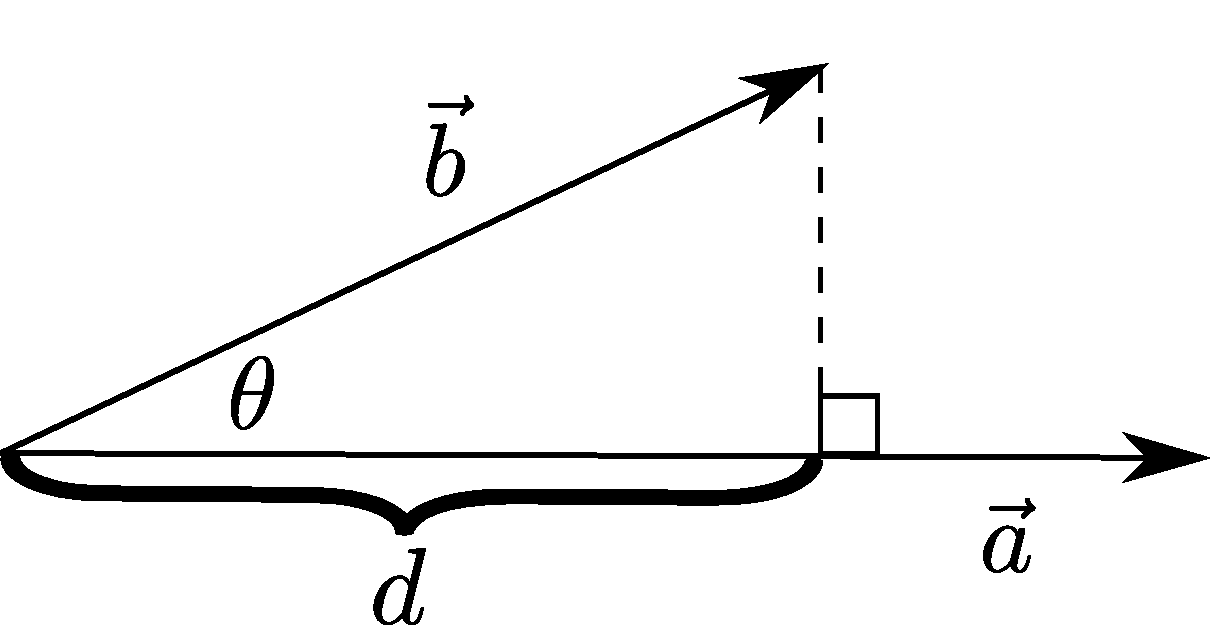
\includegraphics[width=2in]{T3-proj}
    \end{flushleft}
    
    This is basically an exercise in right-triangle trig: $d$ is the length of the side adjacent to the angle, so $\cos\theta = \dfrac{d}{\len{\vec{b}}}$, or $d=\len{\vec{b}}\cos\theta$. On the other hand, we know that $\vec{a}\dotp\vec{b}=\len{\vec{a}}\len{\vec{b}}\cos\theta$, so 
    \[
    d=\len{\vec{b}}\cos\theta = \frac{\vec{a}\dotp\vec{b}}{\len{\vec{a}}},
    \]
    as required. 
    \item Show that
    \[
    (\vec{u}+\vec{v})\dotp (\vec{u}-\vec{v}) = \len{\vec{u}}^2-\len{\vec{v}}^2
    \]
    for any vectors $\vec{u}$, $\vec{v}$ in $\R^3$.
    
    \bigskip
    
    Since the dot product satisfies the distributive property, we can multiply out the left-hand side as follows:
    
    \begin{align*}
    (\vec{u}+\vec{v})\dotp(\vec{u}-\vec{v}) & = \vec{u}\dotp\vec{u}-\vec{u}\dotp\vec{v}+\vec{v}\dotp\vec{u}- \vec{v}\dotp\vec{v}\\
    & = \len{\vec{u}}^2-\vec{u}\dotp\vec{v}+\vec{u}\dotp\vec{v}-\len{\vec{v}}^2\\
    & = \len{\vec{u}}^2-\len{\vec{v}}^2.
    \end{align*}
    Note that we've used the properties $\vec{u}\dotp\vec{u}=\len{\vec{u}}^2$ and $\vec{v}\dotp\vec{u}=\vec{u}\dotp\vec{v}$ to simplify the above.
\end{enumerate}
  
\end{document}